\section{A Method for Length of Life with Reference to the Lot of Fortune and its Ruler (3K,4P)}

\textbf{/260P/} I cannot tell whether the Ancients, although knowing the efficacy of forecasting, were driven by envy to hide this art because of their vainglory and because the human mind finds this art difficult; or whether they spoke in such riddles even though they had not, in fact, grasped what Nature had created, had prescribed, and had bestowed abundantly on mankind after sealing it with Fate. Of all the lovely elements of the numerous great creations in the world, none seems to me to have been begrudged by God for man’s daily use. God would not have revealed it if He had not wished to provide it for use. In contrast men have revealed this art only as they wished or as they were able. As a result, when I read over their chapter <on the following topic>, I wonder at the crookedness and the obscurity of their thought. But I reveal whatever I have discovered by my experience, and in addition, I do not wish to conceal whatever I have gone on to
discover <after writing my previous pages>—this because of the remarkable quality of many forecasts, both good and bad, those happening in a short time or those remaining for a time at a steady state.

Now the following subdistribution will instruct diligent scholars. I have explained it in minute detail since I consider it superior to any other and since I wished to embellish the topic in every way. A general treatment displays a vague outline of details and is easily refuted because of the undisciplined thinking of its students. Let no one shrink away because this chapter is complex, multifaceted, with many rules, but let my reader divinize his nature. For although many <astrologers> have composed many systems, they have put together no solid system.

Now then to the task at hand. The fatal critical points must be determined just as I have directed in my book \textit{The Length of Life}. Now I will clarify this topic more precisely. The chronocratorships are composed of three factors, minimum, mean, maximum. \textbf{/273K/} I have found their determination to be as follows: calculate the periods of the stars and the rising times of the signs from the Lot of Fortune and its ruler, first by hours, then by days, months, and years; or calculate hours for some, days for others, months for others, and years for still others; or using the stars at the angles and rising \textbf{/261P/} and in their proper configurations, calculate first days, then months, then the periods. For men who are already in the prime of life it is possible to allot periods and rising times; for infant nativities begin with the shortest units.

\begin{wrapfigure}[13]{R}{7cm}
\centering
\vspace{-10pt}
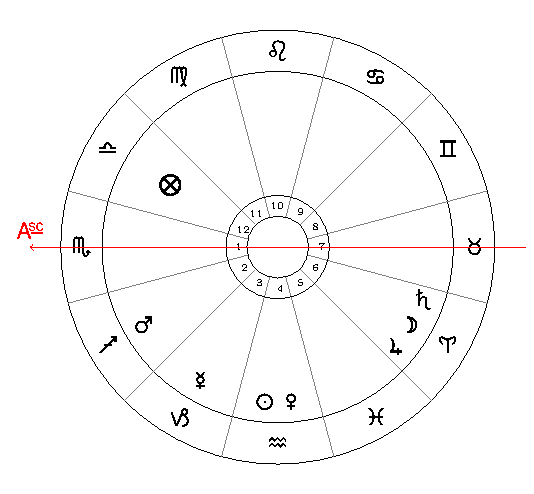
\includegraphics[width=.68\textwidth]{charts/7_4_1}
\caption{Chart 77 [VII.4.1, GH L173]}
\label{fig:chart77}
\end{wrapfigure} 

\noindent For example: \Sun, \Venus\xspace in \Aquarius, \Moon, \Jupiter\xspace in the beginning of \Aries, \Saturn\xspace in \Aries, \Mars\xspace in \Sagittarius, \Mercury\xspace in \Capricorn, Ascendant in \Scorpio, \Fortune in \Libra, klima 6\footnote{\textit{Greek Horoscopes} dates the chart to February 3, 173 CE about midnight}. 

\noindent The allotting stars are \Venus\xspace because of \Libra, \Saturn\xspace because \Venus\xspace is in \Aquarius, \Mars\xspace because \Saturn\xspace is in \Aries. 

\noindent Next I calculated according to periods and rising times, first hours, then days, then months, as follows: I took for \Libra\xspace <=\Venus> 8 days 8 hours, plus the rising time of \Libra (in klima 6) 43 hours. Since \Venus\xspace is in \Aquarius\xspace <house of \Saturn>, I took 57 hours for \Saturn. Since \Saturn\xspace is in \Aries\xspace <house of \Mars>, I took 15 hours for \Mars. The total is 8 days, 123 hours. Now 123 hours equals 5 days 3 hours, and so the grand total is 13 days 3 hours. He lived 13 days 3 hours.

\begin{wrapfigure}[14]{R}{7cm}
\centering
\vspace{-10pt}
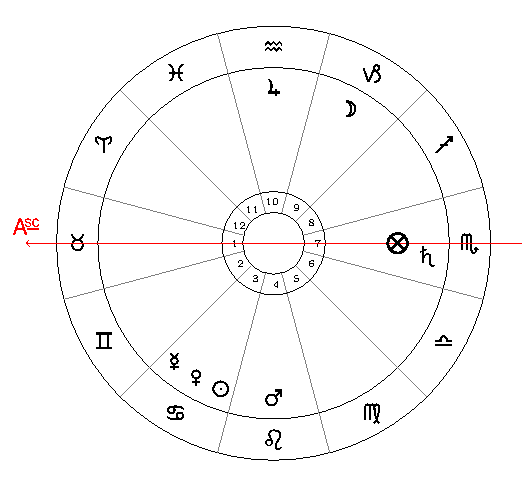
\includegraphics[width=.68\textwidth]{charts/7_4_2}
\caption{Chart 78 [VII.4.2, GH L159]}
\label{fig:chart78}
\end{wrapfigure} 

Another example: \Sun, \Venus, \Mercury\xspace in \Cancer, \Moon\xspace in \Capricorn, \Saturn\xspace in \Scorpio, \Jupiter\xspace in \Aquarius, \Mars\xspace in \Leo, Ascendant in \Taurus, \Fortune\xspace in \Scorpio\footnote{\textit{Greek Horoscopes} dates the chart to July 18, 159 about 2 a.m.}, its ruler <\Mars> in \Leo, and <\Leo´s> ruler <\Sun> in \Cancer. He lived longer than the hours and the days of the periods of the stars plus the rising times of the signs, and so I calculated the months as the third option. 

For \Mars\xspace I took 66 months plus 15, and for the \Sun\xspace in \Cancer <=\Moon> I took 25 months. The total is 106 months, which is 8 years, 10 months. (I submit these nativities as examples; it is also necessary to note the houserulers and the places to see
if they are controlled or opposed by malefics or happen to be out of their sects. Follow all the other directions too.)

\newpage
\begin{wrapfigure}[14]{R}{7cm}
\centering
\vspace{-10pt}
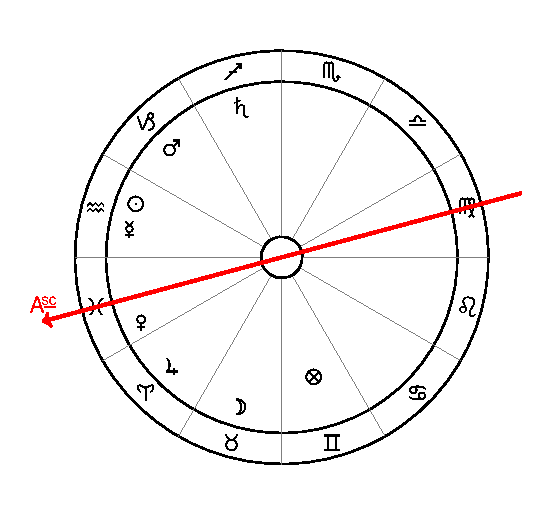
\includegraphics[width=.68\textwidth]{charts/7_4_3}
\caption{Chart 79 [VII.4.3, GH L162]}
\label{fig:chart79}
\end{wrapfigure} 

Another example: \Sun, \Mercury\xspace in \Aquarius, \Moon\xspace in \Taurus, \Saturn\xspace in \Sagittarius, \Jupiter\xspace in \Aries,
\Mars\xspace in \Capricorn, \Venus, Ascendant in \Pisces, klima 6, \Fortune\xspace in \Gemini\footnote{\textit{Greek Horoscopes} dates the chart to February 9, 162 CE about 8 a.m.}. 

I took the months for \Mercury\xspace <ruler of \Gemini> and since \Mercury\xspace is in Aquarius, I took the rising time for \Aquarius, 23 months, plus 33 months for \Sagittarius, since \Saturn\xspace is in \Sagittarius. \textbf{/274K/} Altogether the months total 132, which is 11 years. He died at that age. 

We can find the precise number of days and the precisely measured hours by taking 1/12 of the period of each star. Stars which are appropriately configured with each other and in the same sect can combine their allotments. 

\newpage
\begin{wrapfigure}[14]{R}{7cm}
\centering
\vspace{-10pt}
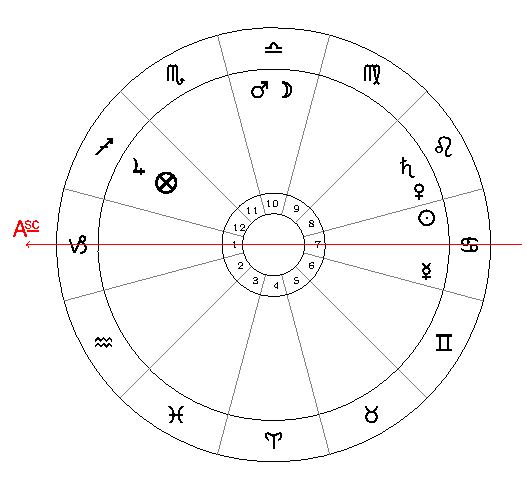
\includegraphics[width=.68\textwidth]{charts/7_4_4}
\caption{Chart 80 [VII.4.4, GH L122, VI.30]}
\label{fig:chart80}
\end{wrapfigure} 

For example: \Sun, \Mercury\xspace in \Cancer, \Moon, \Mars\xspace in \Libra, \Saturn, \Venus\xspace \textbf{/262P/} in \Leo, \Jupiter\xspace in \Sagittarius, Ascendant in \Capricorn, klima 6, \Fortune\xspace in \Sagittarius\footnote{\textit{Greek Horoscopes} dates the chart to June 30, 122 about sunset}. 

The ruler of \Sagittarius, \Jupiter, was located at the Lot. So it allotted the rising time of \Sagittarius, 33 years, plus its own period, 12 years, for a total of 45. \Saturn\xspace trine with \Jupiter\xspace added its period, 57 months, to the previous amount for a total of nearly 50 years. He died at that age. If anyone calculates the rising time of \Leo, 38 months, plus the period of the \Sun, 19 months, he will find the same number of months.

I have submitted these nativities after testing them by personal experience. If anyone wishes to test this method using a mere hearsay nativity, he will not find it to be valid. Note that different critical points
are indicated whenever the chronocratorship of a malefic in configuration and in aspect takes control. The same caution applies to the Ascendant and its ruler, whenever the stars happen to be succeeding to or yielding the chronocratorship, if the Lot of Fortune and its ruler are not operative.

\newpage